\chapter{Materials and Methods}
\section{Data Description}
	Present research is based on heterogeneous behavioral data describing animals from seven different cohorts. Each cohort, having various number of animals of the same sex, was independently undergoing the ethanol self-administration experiment under standardized protocol described later in the text.
	
	\subsection{Animals}
	Fifty rhesus monkeys (Macaca mullata) from the Oregon National Primate Research Center (ONPRC) were used in this study. Animals were both male and female and derived from seven cohorts, designated as ``4", ``5", ``6a", ``6b", ``7a", ``7b", and ``10". Each cohort had animals of the same sex. Table~\ref{tab:data-breakdown} displays the sex of the monkeys corresponding to each cohort, their average age in years, average weight in kilograms, and age at first intoxication, i.e., age when their BEC (Blood Ethanol Concentration) was greater than 80 mg/dl \shortcite{dawson2008age, li2007alcohol}. In the table, \textbf{N} represents the total number of monkeys per cohort and \textbf{n} represents the overall number of monkeys in our analysis.
	
	\begin{table}[htb]
		\centering
		\caption{Breakdown of cohorts used in this study. Weight is the daily average during induction. Age at intoxication is defined as the first BEC over 80 mg/dl.}
		\label{tab:data-breakdown}
		\begin{tabular}{lllllc}
			\hline
			\abovespace\belowspace
			Cohort & N (n=50) & Sex & Age (yrs) & Weight (kg) & Age at intox. (yrs) \\
			\hline
			4 		   & 10 & M & 10.13 & 9.61 & 8.64   \\
			5            & 8 & M & 7.2 & 9.34 & 6.05  \\
			6a           & 6 & F & 5.36 & 5.36 & 4.23 \\
			6b    		& 5 & F & 7.05 & 6.76 & 5.91  \\
			7a           & 8 & M & 5.84 & 8.44 & 4.76   \\
			7b    		& 5 & M & 7.21 & 11.08 & 6.01   \\
			10    		& 8 & M & 6.76 & 5.26 & 5.48   \\ 
			\belowspace \\
			\hline
		\end{tabular}
	\end{table}

	All animals were born into a pedigreed population and remained with their mothers in a multigenerational troop until weaning at about two years of age. All monkeys were continually in a social setting at Oregon National Primate Research Center (ONPRC) and transitioned to individual cages within a laboratory building at least three months prior to the onset of ethanol self-administration according to established protocols \shortcite{helms2014effects}. The age range encompasses late adolescence to early middle age of captive monkeys and data from a subset of these monkeys addressing age as a risk factor for chronic alcohol self-administration has been published \shortcite{helms2014effects}.
	
	Monkeys were housed individually with four cages arranged on a single rack: two cages located above and two below. Monkeys that weighed over 10kg were allowed access to both horizontal cages, but only one drinking panel was affixed to the side of the cage. Each cohort was housed together in the room using multiple racks. All animals had visual and auditory access to other monkeys in the room. Male monkeys were allowed tactile access to adjacent monkeys through grooming grids inserts in the common wall of the cage and female monkeys were allowed two-hour access/day to a common space by removing the horizontal barriers between the cages.
	
	
	\subsection{EtOH Self-Administration Experiment Description}
	The monkeys were induced to self-administer 4\% EtOH (mixed with water) using a schedule-induced polydipsia (SIP) procedure previously described in detail \shortcite{vivian2001induction, grant2008drinking}. Visual representation of the experiment is shown in Figure~\ref{experiment_design}. The dose of EtOH the monkeys were required to consume each day increased every 30 days beginning from 0.5 g/kg to 1.0 g/kg, and finally to 1.5 g/kg. These three stages of 30 days each formed the \textbf{induction} phase.
	
	After the $30^{th}$ session of 1.5 g/kg EtOH the monkeys had concurrent access to EtOH (4\% mixed with water) and water. In other words, animals were to choose between water and alcohol solution. Access was limited to 22 hours a day ensuring animals would have guaranteed sleep time. This phase, when animals had a free choice of drink, was termed \textbf{Open Access (OA)}. Duration of OA varies for each cohort (from six months to 18 months); food, as at least 3 meals per day, was provided during OA \shortcite{grant2008drinking}.
	
	\begin{figure}[ht]
		\centering
		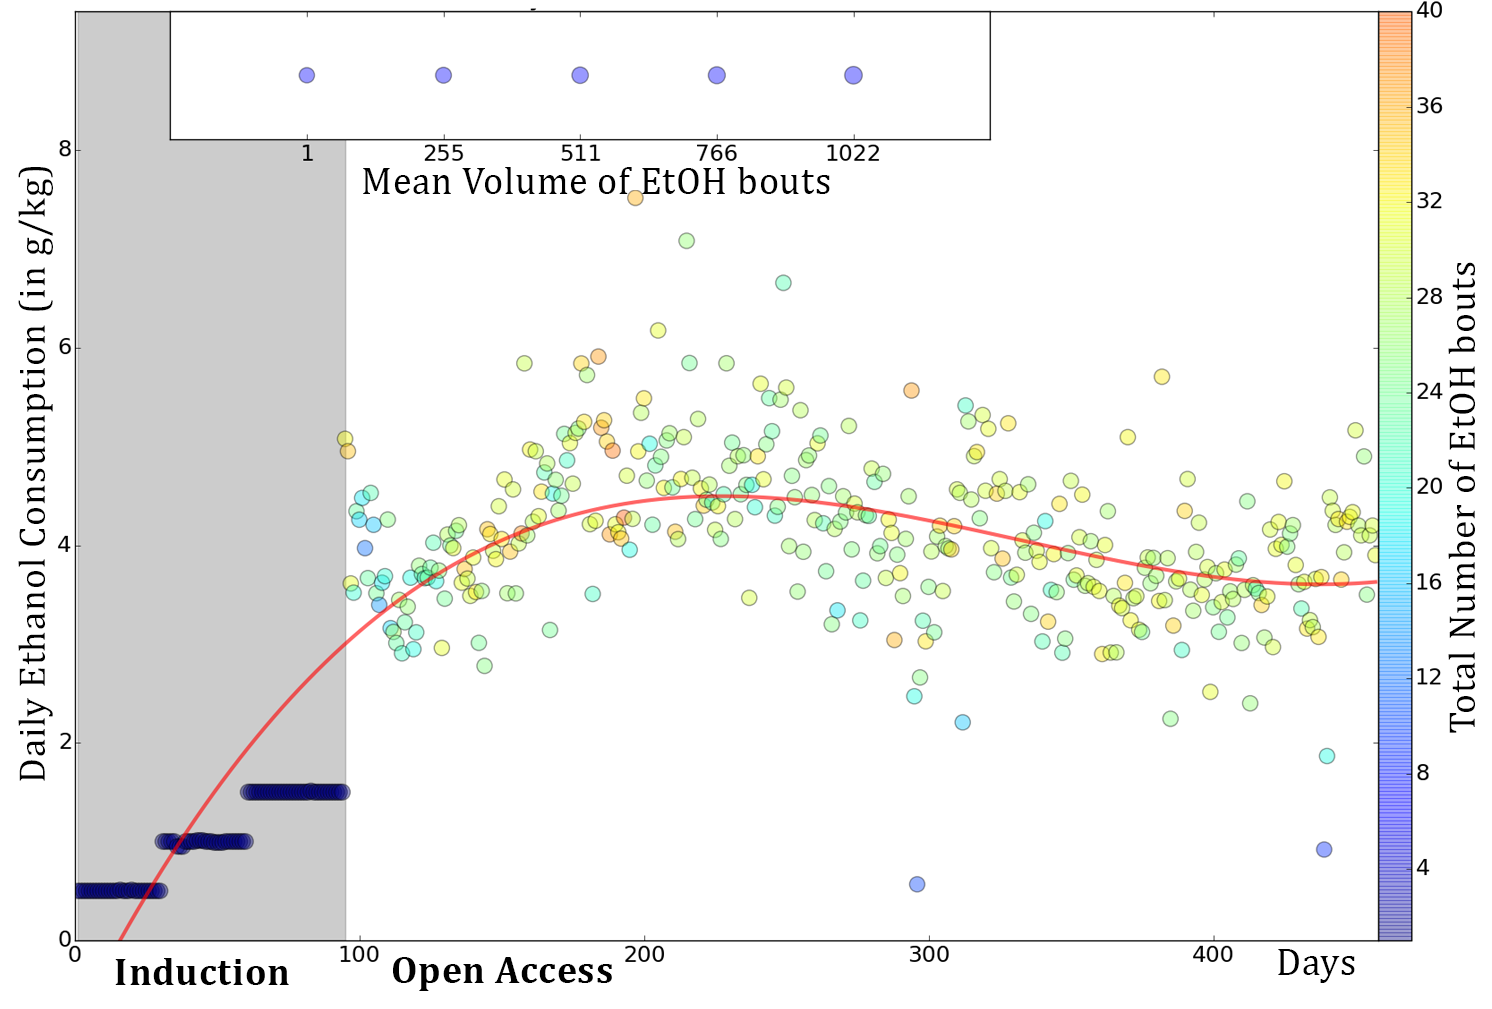
\includegraphics[width=1\linewidth]{figures/experiment_design.png}
		\caption{EtOH self-administration experiment design illustration for one animal. Shaded area represents Induction phase. The rest is Open Access (OA). Points represent aggregated information about one drinking day. A point's position on the Y-axis shows average ethanol consumed that day. The size of the point represents mean volume of ethanol bouts, while color indicates the total number of such bouts during that day.}
		\label{experiment_design}
	\end{figure}
	
	\subsection{Dataset Structure}
	Throughout the experiment magnitude of measurements for food and liquid consumption were taken on daily basis. At the end of the day some attributes were aggregated into mean values, which were more convenient for analysis. Raw data was also stored, which proved to be useful whenever new metric was adopted. 
	
	In earlier research \shortcite{baker2014chronic}, described in chapter 2, \textbf{Drinking Categories (DC)} were assigned to each animal based on quantitative data \textit{during the open access phase}. It was shown that clustering all animals into four DCs (low drinking (LD), binge drinking (LD), heavy drinking (HD) and very heavy drinking (VHD)) captures the most variability of quantity/frequency measures of alcohol intake. The important caveat, however, is that these \textit{DCs are not innate features of the animals, but an arbitrary assigned labels}, which do not necessarily constitute the objective reality. Nevertheless, for the purposes of our research DC serves as an objective function, thus in this paper we treat drinking category labels as the ground truth.
	
		\subsubsection{Drinking Behavior Attributes}
		Present research uses data recorded from approximately 5000 total sessions (over 20 GB of normalized data in the database), one session per day per animal. During every session, detailed information about different relational quantitative attributes was collected for behavioral analysis. Daily averages and other derived attributes were summarized into daily averages as appropriate \shortcite{grant2008drinking}.
		
		Figure~\ref{experiment_design} provides an illustration of the data collected for one animal. Points represent aggregated information about one drinking day: average ethanol consumed, mean volume of ethanol bouts and the total number of such bouts.
		
		Table~\ref{data-selected-attributes} shows a partial list of drinking attributes that explain most of the variation in the data and provided the greatest predictive power, according to the methods described herein. A complete list of all the attributes studied in our research can be found in the Appendix A, Table~\ref{data-all-attributes}. In addition to these quantitative measurements in seconds, milliliters or percentage points, there are several qualitative attributes, which we model with dummy variables.
		
		\begin{table}[!t]
		\centering
		\caption{Partial set of database attributes describing animal drinking behavior during induction. Each variable was summarized daily for 90 days. A complete list is available in the Appendix A, Table~\ref{data-all-attributes}.}
		\label{data-selected-attributes}
		\begin{tabular}{ll}
			\hline
			\abovespace\belowspace
			Drinks (intakes $\le$ 5 sec apart)&	Bouts (intakes $\le$ 5 minutes apart)\\
			\hline
			Number of EtOH drinks& 	Number of EtOH bouts\\
			Average EtOH drink length (sec)&	Average EtOH bouts length (sec)\\
			Average EtOH drink volume (ml)& 	Average EtOH bouts volume (ml)\\
			Median EtOH inter-drink interval (sec)& Median EtOH interbout interval (sec)\\
			Average number of EtOH drinks per bout& Number of H2O bouts\\	 	 
			\belowspace \\
			\hline
			\abovespace\belowspace
			First and Max bout &	Time \& Other \\
			\hline
			Number of EtOH drinks in first bout& Time to reach EtOH allotment (sec) \\
			\% of days EtOH consumed in first bout& Latency to first EtOH drink (sec) \\
			Max bout volume (\% of day's total EtOH) & Number of bouts with max EtOH \\
			Max bout length (sec) &	EtOH in first 10 min. (\% of day total)\\
			Sequence number	of max bout & Average number of H2O drinks in bout \\	 	 
			\belowspace \\
			\hline
		\end{tabular}
		\end{table}

	\subsection{Data Consistency}
	Most of the data was collected using automated processes, which ensured the overall quality and consistency of the data. However, there were two major sources of errors and inconsistency which we had to address: human and machine errors, and natural inconsistency.
	
		\subsubsection{Human and Machine Errors}
		Humans were partially responsible for data aggregation, leading to occasional errors. Lab employees also were to control the environment settings which may produce unplanned variation. Since MATRR absorbs the data from multiple labs and various sources not following data guidelines is an issue. Usage of different operation systems created another set of compatibility problems since data partially were sent into the database in form of spreadsheets. Overall, we tried to spot and fix such errors, if possible, and not to use inconsistent data otherwise.
		
		\subsubsection{Natural Variation versus Inconsistency}
		Since the data describes animal behavior we needed to be careful to distinguish between random natural inconsistencies and variables of interest. For example, animals undergoing a blood drawing are very stressed, which affects alcohol consumption; when animals are sick they change their behavior. These cases may lead to data inconsistency which we want eliminate. On the other hand, females vary their drinking pattern in correlation with the menstruation cycle (this would be further described in the chapter four) which we want to account for.
		
		To ignore the data inconsistency that we can not fix we created exception days which are not used in the studies.
	  
\section{Computational Tools}
	This section presents the parts of the computational apparatus used in this research, their interaction, and their advantages and limitations.
	\subsection{Monkey Alcohol and Tissue Research Resource}
	The Monkey Alcohol and Tissue Research Resource \nobreakdash{(MATRR)}
	is a web system developed primarily in the Python programming language. MATRR was created to store tissues from EtOH and control subjects, empirical data relating to alcohol self-administration, data
	derived from tissue analysis, and data analytics (including data
	mining and data harmonization, and tissue dissemination) \shortcite{daunais2014monkey}. 
	The MATRR serves to close the loop between
	tissue derived from this oral alcohol self-administration model
	and integrated analysis of behavioral, physiological, pharmacological,
	and molecular data by tracking analyses conducted on
	distributed tissues, thus reinforcing tissue selection and experimental
	development by a network of laboratories. Metadata about all animals described in this study, as well as raw and
	semi-processed drinking and behavioral data, are imported in
	MATRR (http://www.MATRR.com) where analysis is performed.
	
	\subsection{Hardware}
	All computations were executed on MATRR’s web and database
	servers. These are twin machines, each running 4 Intel Xeon E5620
	(2.4 Ghz) with 4 cores each, 47 GB RAM, and 1.7 TB disk space in
	a RAID configuration. The hardware design ensures efficiency of the calculations while providing security against the data loss by using non-volatile storage. 
	
	\subsection{Object-Relation Mapping}
	MATRR uses PostgreSQL DBMS, one of the most advanced and efficient open source databases available. All the data manipulation is done via Object-Relation Mapping (ORM) within Django. Django is a high-level Python Web framework that encourages rapid development and clean, pragmatic design. Django includes connectors to the PostgreSQL and allows a developer to treat the relations in the database as if they were objects, and tuples of the relations as if they were object instances. This greatly simplifies and speeds up the data analysis. In conjunction, the advanced DBMS is capable of storing huge datasets as a set of normalized relations securely on non-volatile storage while scientist works with such data as if it was all in the main memory, without any complexity of converting and aggregating data using the Structured Query Language.  
	
	
	\subsection{Data Analysis Tools}	
	\textit{SciPy} is a Python-based ecosystem of open-source software for mathematics, science, and engineering \shortcite{millman2011python}. Present research greatly benefited by using several of its core packages such as Numpy, Pandas and Matplotlib. Numpy was used for efficient statistical computations of mean, variance and correlations.
	
	\textit{Pandas} is an open source, BSD-licensed library providing high-performance, easy-to-use data structures and data analysis tools for the Python programming language \shortcite{mckinney-proc-scipy-2010}. Pandas was created because native Python is great for data preparation, but does not readily accommodate data analysis and modeling. Pandas enables us to carry out entire data analysis workflow in Python without having to switch to a more domain specific language like R. Pandas, however, does not implement significant modeling functionality outside of linear and panel regression, thus present research uses Statsmodels and Scikit-learn libraries.
	
	\textit{Statsmodels} is a Python module that allows users to explore data, estimate statistical models, and perform statistical tests \shortcite{statsmodels2010}. An extensive list of descriptive statistics, statistical tests, plotting functions, and result statistics are available for different types of data and each estimator. Present research took advantage of the Statsmodels' implementation of generalized linear models, validation methods and various statistical tests. 
	
	\textit{Scikit-learn} is an open source Python library containing simple and efficient tools for data mining, machine learning and data analysis \shortcite{scikit-learn}. In particular, present research used the following Scikit-learn implementation of the following models: Support Vector Machines, Random Forests, Gradient Boosting Classifier and Regressor, and others. 
	
	It is worth noting that all the libraries above are easy to use in combination with each other which renders a powerful ecosystem for the fast and efficient data analysis which does not require any costly software licensing. 
	
	\subsection{Visualization Tools}
	\subsubsection{Visualization Libraries}
	All visualizations in this paper were made using Matplotlib and Seaborn python libraries. 
	
	\textit{Matplotlib} is a python 2D plotting library which produces publication quality figures in a variety of hardcopy formats and interactive environments across platforms \shortcite{Hunter:2007}. The Matplotlib community provides a magnitude of examples from scientific research along with the constant improvements and new features. Most of the features of the R (statistical language) visualization library ggplot2 are now available in Matplotlib, which allows the combined flexibility and coverage of the proven statistical techniques from R and computational efficiency and scalability of python.  
	
	\textit{Seaborn} is a Python visualization library based on matplotlib. It provides a high-level interface for drawing attractive statistical graphics \shortcite{michael_waskom_2014_12710}. Seaborn greatly facilitates data analysis by providing easy to use visualization methods for most popular and useful statistical tools. 
	
	\subsubsection{Visualization Techniques}
	Along with the standard histograms, scatterplots and boxplots some more advances visualization techniques were used.
	
	\textit{KDE plot} allows efficient display of univariate and bivariate kernel density estimation plots in form of curve or contours. KDE plots smooth the data points facilitating clear focus data consistencies or anomalies. This in turn allows researches to closer investigate the data and generate hypothesis.
	
	\textit{Violin plot} is a box and whisker plot with a rotated KDE plot on each side \shortcite{hintze1998violin}. It shows the distribution of quantitative data across several levels of one (or more) categorical variables such that those distributions can be compared. Unlike a box plot, in which all of the plot components correspond to actual datapoints, the violin plot features a kernel density estimation of the underlying distribution \shortcite{michael_waskom_2014_12710}.
	
	\textit{Hexagonal Bin (hexbin) plot} is a useful alternative to the scatterplots in situations when there are too many data points to be easily perceived. In other words, if the data is too dense to plot each point individually, it is useful to combine close by points into the bins. Consequently, bins are plotted with varying color indicating the number of occurrences.  
	Another way to look at the hexbin plots is as an 2D extension of the histograms. In this manner we are able to capture the distribution along two dimensions simultaneously. 
	
	\subsection{MVC Approach In Data Analytics}
	Model-view-controller (MVC) software architectural pattern  approach is an accepted standard in modern software development process \shortcite{reenskaug2009dci}. Present research greatly benefited by applying similar principles for data analysis. Usually the same data aggregation, though differently unfolded, was needed for different analysis tools, each of which offered various visualization options. Consider Table~\ref{tab:bec-domain-options}, which shows the domain of options for ``BEC $\sim$ EtOH" study, discussed in chapter four.
	
	\begin{table}[h]
	\centering
	\caption{Domain of options for data analysis}
	\label{tab:bec-domain-options}
	\begin{tabular}{lp{3in}}
	    \hline
	    \abovespace\belowspace
	    Variable & Domain \\
	    \hline
	    Schedule & 22 hours session, daylight   \\
	    Factor & Intoxication over 80 mg BEC, BEC outside of two standard deviations (stdev), BEC more than two stdev.   \\
	    Visualization format & 24 separate panels, 12 combined panels   \\
	    ANCOVA slope equality test & Yes, no   \\
	    Aggregate with hexbin & Yes, no  \\
	    \belowspace \\
	    \hline
	\end{tabular}
	\end{table}
	
	Such comprehensible analysis layout, along with the massive data volumes and its heterogeneity creates a need for an efficient data analysis system, which consists of interchangeable blocks of code, related to data retrieval and aggregation, data slicing and filtering, and visualization.  Below is an overview of the system created for present paper.
	
	A data layer, responsible to retrieve the actual data from the PorstgreSql database, was implemented with the aid of Django ORM tools. Django allows the treatment of huge chunks of raw data in the database as if it is actually stored in main memory as an object instance. The speed of retrieval from the disk is greatly affected by the number of filters and aggregations involved as well as the chosen algorithms. Therefore, separate Python functions were written to retrieve, filter and aggregate the data in the most efficient way and store it in the intermediate temporary files. These files were later used for various analysis techniques. 
	
	The controller layer is handled by Pandas which allows us to slice and dice data facets easily and efficiently. Pandas consumes temporary aggregated files and produces views for the current experiment. Again, Python functions are written in such a manner that should a researcher have a new idea for data analysis within the same study, only a small piece of code need be appended into the codebase. Python allows to pass functions as an argument of another function which makes it very easy an intuitive to build the data analysis system as a set of interchangeable building blocks with the common API. 
	
	Lastly, the view layer is handled by Matplotlib and Seaborn. To make a new visualization, one has to only write a new visualization function which implements the API given by the controller and need not to worry about integration of this new visualization in different parts of the data analysis system. 	
	
\section{Analytical Tools}
	In this section analytical tools used in the paper are briefly described.
	\subsection{Correlation Analysis}
	\textit{Pearson product-moment correlation coefficient} is used to capture correlation as a statistical relationship between two random variables or two sets of data. The limitation of Pearson coefficient is that it is sensitive only to a linear relationship between two variables.
	
	\textit{Analysis of Covariance (ANCOVA)} is a general linear model which evaluates whether population means of a dependent variable are equal across levels of a categorical independent variable, while controlling for the effects of other continuous variables that are not of primary interest, known as covariates. \shortcite{keppel1991design} Intuitively, ANCOVA could be thought of as a blend of ANOVA and linear regression, which allows us to compare two regressions on whether or not the sample slopes are estimates of the same population slope. 

	
	\textit{Kernel Density Estimation (KDE)} is a non-parametric way to estimate the probability density function of a random variable \shortcite{rosenblatt1956remarks}. Such estimation, or smoothing, facilitates inferences about the population, based on a finite data sample. Gaussian kernel was chosen for its simplicity and effectiveness with multivariate distribution. 
	
	\subsection{Locally Weighted Linear Regression \label{lwlr}}
	\textit{Locally Weighted Linear Regression (LWLR)} is a useful tool for greatly enhancing the visual information on a scatterplot by computing and plotting smoothed points with little additional computational cost \shortcite{cleveland1979robust}. LWLR is the extension of the simple linear regression model shown in Equation~\ref{eq:lr-model}:
	\begin{equation}
	Y=X\beta+\epsilon
	\label{eq:lr-model}
	\end{equation}
	
	The solution for linear regression, expressed in the closed (matrix) form, is shown in Equation~\ref{eq:lr-solution}:
	\begin{equation}
	\beta =(X'X)^{-1}X'Y
	\label{eq:lr-solution}
	\end{equation}
	
	To smooth the data points, LWLR introduces the weight matrix $W$, as shown in Equation~\ref{eq:lwlr-solution}:
	\begin{equation}
	\beta =(X'WX)^{-1} X'WY
	\label{eq:lwlr-solution}
	\end{equation}
	
	Such weight matrices are computed via the kernel smoothing using the nearby data points. Gaussian kernel was used in the present study, as shown in Equation~\ref{eq:lwlr-weights}:
	\begin{equation}
	w^{(i)}=\exp(-\frac{||x^{(i)} - x||^2}{2\tau^2})
	\label{eq:lwlr-weights}
	\end{equation}
	
	This technique smooths each data point using neighbor points in such a way that closer points have more influence than those that are further away. Exactly how far away each point influences the others is regulated by the bandwidth parameter $\tau$ - the ``narrowdness" of the Gaussian ``bump". Choosing the appropriate value for $\tau$ is  essential for a good smoothing: too big value will result in the straight line (converges to the simple linear regression); too small value will result in overfitting and wrong predictions. Although there are some heuristics for automated choice of $\tau$, in this research we used an arbitrary value which demonstrated the best visual experimental results. 
	
	LWLR with the careful choice of $\tau$ is a robust fitting procedure and guards against deviant points distorting the smoothed points, rendering it useful in ``noisy" heterogeneous datasets with often occurring data inconsistencies. 	
	
	\subsection{Accuracy Evaluation \label{section:accuracy-evaluation}}
	This section briefly presents the tools used in research to validate the model, evaluate classification accuracy and performance. The goal of model validation is to assess how the resulting trained classification model will generalize to an independent new data set. In our settings that means to validate how well the model trained to classify very heavy drinkers on 50 animals would perform on new unseen animals of the same species and undergoing the same experiment. Because of the small data sample size of 50, we always used exhaustive cross-validation.
	
	\textit{K-fold} cross validation technique was used as the primary classification accuracy evaluation method. The idea is to randomly distribute data among the K folds and iteratively train the model on K-1 of them, leaving one fold for validation.  This approach avoids sacrifices of a single training-testing data split and allows for more statistically robust accuracy measure. 
	
	K was chosen to be 10 to produce folds of equal size (our sample size is 50). Since data is randomly distributed among folds, we run cross validation 20 times on each task to ensure the result is not due to the chance. Thus the mean of the 20 runs of 10-folds cross validation was always used as a reported accuracy. 
	  
	\textit{A leave one out} method was used in addition to K-fold cross validation technique. The idea is essentially the same as of K-fold, but with K equal to the sample size. Leave one out cross validation can be computationally costly thus it was used only for measuring accuracy within the cohorts, which have a non-constant number of animals rendering the usage of the K-fold to be problematic. 
	 
	\textit{A confusion matrix} is a specific table layout that allows visualization of the performance of an supervised learning algorithm. Each column of the matrix represents the instances in a predicted class while each row represents the instances in an actual class (or vice-versa) \shortcite{powers2011evaluation}. The name stems from the fact that it makes it easy to see if the system is confusing two classes (i.e. commonly mislabeling one as another). In the present research it was important to analyze what is exactly being mislabeled: LD mislabeled as BD is not crucial (since these drinking category labels are arbitrary by nature), yet LD mislabeled as VHD is significant; however, it could also indicate some innate peculiarity of the animal.  
	
	\subsection{Machine Learning Models \label{section:ml-models}}
	When choosing the model for the classification task we are mainly concerned with the robustness of the model on the small size samples and its resistance to overfitting. Due to the natural noise in the data we needed models that would adequately work with outliers, penalizing them in a manner that does not skew the general view of the data. After an extensive search, several potential models were explored.
	
	\textit{Support Vector Machines (SVM)}, as the model which tries to optimize the bound of the generalization error, depends on the distance from the decision boundary to the nearest point to each class, but is independent of the dimensionality of the features space \shortcite{cawley2007preventing}. SVM provides a flexible means of regularization, thus, given the appropriate kernel parameters and the regularization choice, this model should be resistant to overfitting and produce robust results on small data set.
	
	\textit{Random Forests (RF)} were chosen because they are proven to perform relatively well on small data sets, resisting overfitting by penalizing data outliers without skewing the distribution of the data (Yang et al., 2010). RFs are particularly common in bioinformatics and genomics research, where the number of features can be several orders of magnitude greater than the number of observations. One of the most important qualities of RFs is the possibility of using several distinct low-dimensional prediction models based on small subsets of features that, together, increase classification accuracy (Yang et al., 2010). \shortcite{yang2010review}
	
	\textit{Bootstrap aggregating (Bagging)}, which is not a classification model by itself, but rather a wrapper mechanism that is devoted to reduce variance and avoid overfitting, thus improving the accuracy of the base classifier. The basic idea of bagging is to generate several training sets by the uniform examples' sampling with the replacement. For a sufficiently big sample size each set is expected to have the fraction $1-\frac{1}{\exp}$ ($\approx 63.2 \%$) of unique examples, the rest being duplicates \shortcite{aslam2007estimating}.	The evidence, both experimental and theoretical, is that bagging can push a good but unstable procedure a significant step towards the optimality \shortcite{breiman1996bagging}. 
	
	\textit{Gradient Boosting classifiers} were chosen as an advanced version of random forests. In order to decrease overfitting, gradient boosting introduces regularization through shrinkage providing
	two regularization parameters, the learning rate, \textit{v}, and the number of components, \textit{M}. Each one can control the degree of fit and thus affect the best value for the other one. \shortcite{friedman2001greedy}. To manage the small sample size, gradient boosting has the following feature: at each iteration of the algorithm, a base learner is to be fit on a subsample of the training set drawn at random without replacement \footnote{This is different from bagging, which samples with replacement, in that it uses samples of the same size as the training set.} \shortcite{friedman2002stochastic}.	
	
	\subsection{Partial Dependency Plots}
	Partial dependence plots (PDP) show the dependence between the target function and a set of ``target" features, marginalizing over the values of all other features (the complement features) \shortcite{hastie2005elements}. Due to the limits of human perception the size of the target feature set must be small (usually, one or two) thus the target features are usually chosen among the most important features. 
	
	Intuitively, a single feature does not mandate the category of a monkey, but rather a set of features together may determine the outcome of the target variable, Drinking Category. In order to understand the interaction between features we make use of PDPs. Such plots provide a visual understanding of how two features depend on each other and contribute to determining the drinking category of a monkey. PDPs are a two-dimensional color plot that can be used to inspect the significance of features in the process of categorization of data. Here, PDPs are produced from Gradient Boosting Regressors. 

\section{Improving Models}		
	This section describes mechanisms used in the ``predicting future drinkers" classification study, which is based on machine learning models and data features, as explained below.
	
	\subsection{Feature Generation \label{section:feature-generation}}
	For the purposes of machine learning, the attributes or variables that describe the data are known as features, and are used to train classification models. It is well understood that good features, along with the appropriately chosen model, are necessary to produce good classification results \shortcite{guyon2008feature}. 
	
	Initially we had approximately 90 sessions per animal, each session having around 30 attributes (i.e. day's mean drink volume\footnote{For the full list refer to Appendix A, Table~\ref{data-all-attributes}.}). Each attribute has an absolute\footnote{``Absolute" here does not imply non-negativity, as in mathematics.}  value. This number of measurements for each animal renders usage of plain attributes to be problematic. Additionally, absolute values (as opposed to relative) of plain attributes do not show subject adaptation to the introduced alcohol. That adaptation is the process we want to capture. Thus, we had to reduce the attribute-space dimensionality by generating meaningful and comparable features to feed into our machine learning models. 
	
	The first step removes the logically ineffective attributes. For example, total ethanol consumed was removed because it is the same for every animal since we only analyze induction phase where animals undergo standard schedule and overall alcohol dosage. The second step generates additional attributes, derived from the raw data. For example, the amount of ethanol consumed in the first 10 minutes of the session, as a percentage of the day's total allotment, is a novel parameter not previously used in other studies. 
	
	After attribute filtering and generation, we reduce dimensionality by capturing relative changes in the drinking behavior, steps three and four, and as illustrated in Figure~\ref{features_generation}.
		
	\begin{figure}[ht]
		\centering
		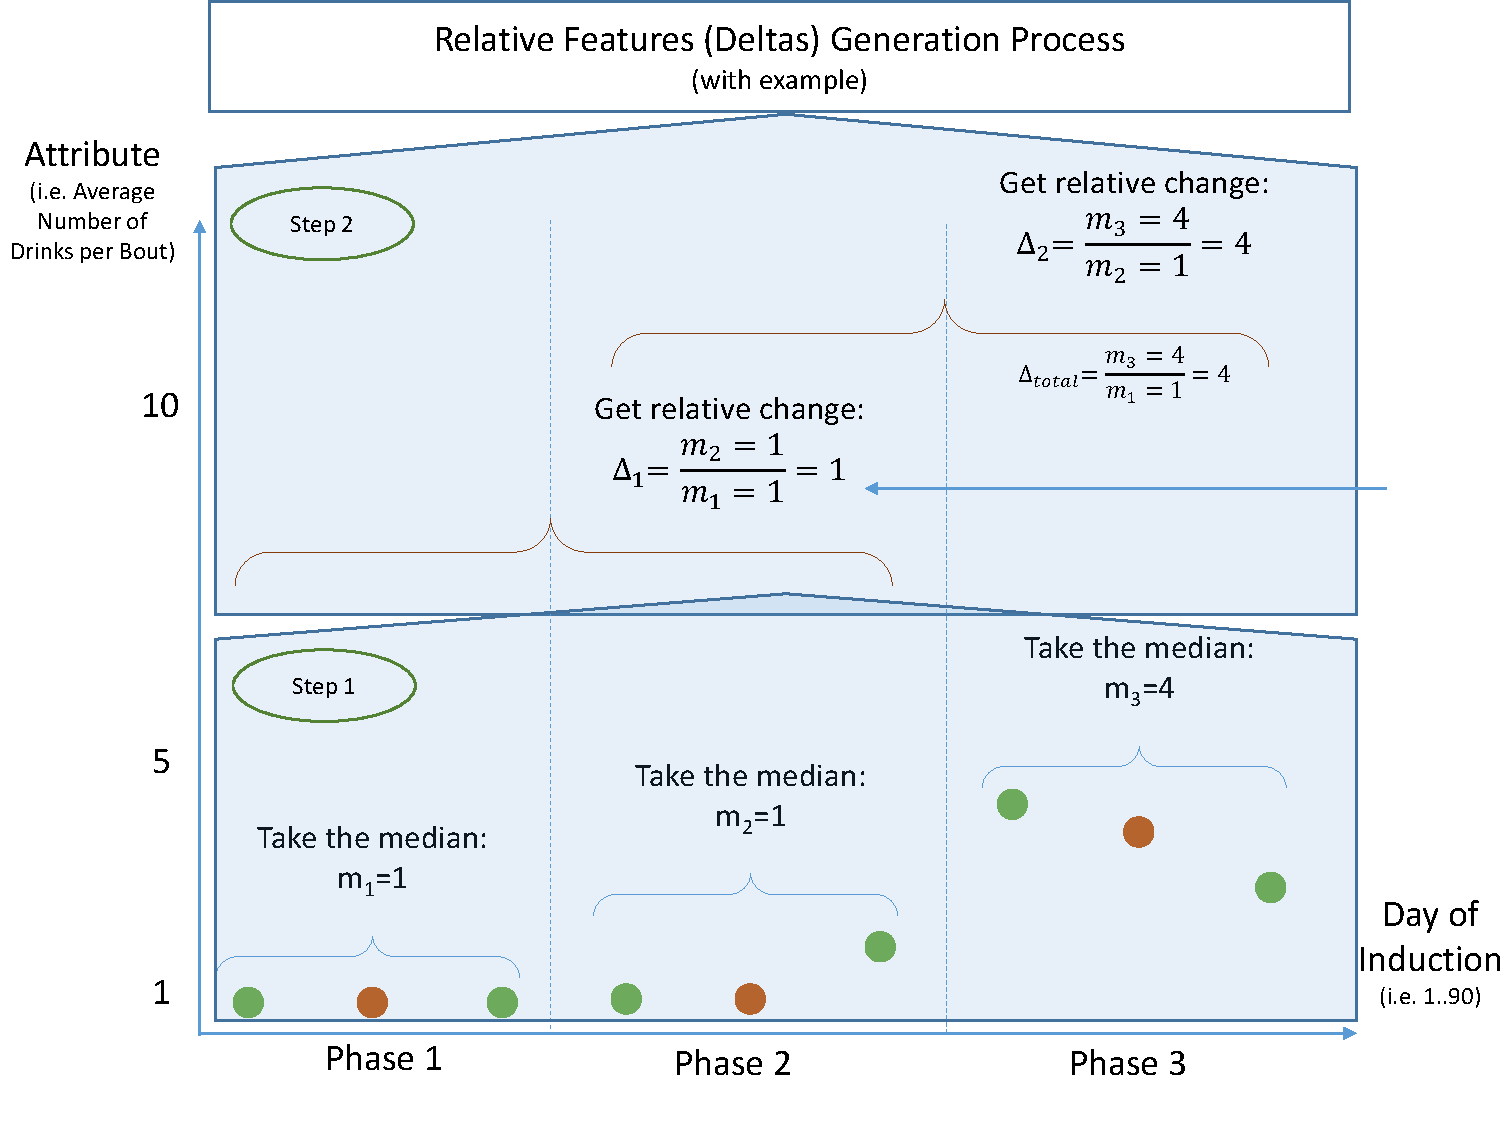
\includegraphics[width=1.1\linewidth]{figures/features_generation.pdf}
		\caption{Relative features (deltas) generation process.}
		\label{features_generation}
	\end{figure}
		
	The third step captures the tendencies of attribute values along the induction time-line. We decided to split 90 days into three stages (which relates to the three different dosage of total ethanol allotment for the day), and to take the central tendency value. Median was chosen because, unlike mean, it alleviates data inconsistency problems, described in the previous section. At the end of this step we had three absolute values for each attribute. We could not compare these values yet, because they \textit{do not indicate the changes in the drinking behavior} of the animal.
	
	The last step makes values comparable by converting absolute values to relative values as formally presented in formula \ref{eq:rel-deltas}. For each attribute, the median of the second stage is divided by the first and median of the third stage is divided by the second yielding two \textbf{relative deltas }, showing by \textit{how much, relatively, an animal changed its alcohol consumption preferences over the course of induction.} 
	
	\begin{equation} \label{eq:rel-deltas}
	\Delta_{ij}^{attr}=\frac{Median(atrr_{stage_i})}{Median(atrr_{stage_j})}, \text{where } i,j=1..3, j \neq j
	\end{equation}
	
	By performing these four steps we created comparable relative deltas that capture changes in the drinking behavior. Consider the example shown in the Figure~\ref{features_generation}: $\Delta_1=1$ indicates no change in behavior regarding this attribute, $\Delta_2=4$ indicates a four-fold increase in preference, which is comparable to the increase by other animals. On the other hand, if all the animals consumed their allotments in the first drink, on average, due to the small size of the allotment, this generated feature (delta) would not show any significance, because each animal would have same value of 1.

	\subsection{Feature Selection \label{section:feature-selection}}
	In addition to good features, machine learning algorithms require an appropriate number of features. Having too many features, especially \textit{if the number of features exceeds the number of observations (n), usually leads to ill-posed models and underdetermined mathematical solutions}. Failure to reduce the dimensionality of the problem by limiting the feature set to those with the highest predictive power can prevent systems from adequately determining which features augment, counteract, or contribute to the eventual outcome \shortcite{barber2012bayesian}.
	
	A forward selection strategy, which we employed in this study to select the most appropriate features, tests a model iteratively, increasing the number of features at each iteration and measuring the accuracy using a K-fold cross-validation \shortcite{alpaydin2014introduction}. Each forward selection iteration adds the feature that gives the best increase in performance in combination with existing features already in a set of chosen features. 

	\subsection{Novelty Two-Step Classification Model}	
	\begin{table}[h]
		\centering
		\caption{Drinking category distribution in cohorts. }
		\label{tab:dc-by-cohort}
		\begin{tabular}{llllll}
			\hline
			\abovespace\belowspace
			Cohort & Sex & LD & BD & HD & VHD\\
			\hline
			Rhesus 4  & M & 5 & 4 & 1 & 0 \\
			Rhesus 5  & M & 0 & 1 & 3 & 4 \\
			Rhesus 6a & F & 0 & 0 & 0 & 6\\
			Rhesus 6b & F & 3 & 9 & 1 & 1\\
			Rhesus 7a & M & 3 & 1 & 2 & 2\\
			Rhesus 7b & M & 3 & 1 & 1 & 0\\
			Rhesus 10 & M & 2 & 3 & 1 & 2\\
			\hline
		\end{tabular}
	\end{table}
	
	Having multiple categories and few observations leads to underdetermined solutions and ill-posed models of classification. Unless we are interested in detection rather than classification, an ideal classification framework contains a larger number of observations than categories and uniform observations within each category. Since the work presented here does not fall into that ideal framework (four categories, 50 observations, and inconsistent observations per category, see Table~\ref{tab:dc-by-cohort}) we reduce the number of categories from four to two and implement a two-step classification process. The first step distinguishes between two combined groups of similar categories: (1) LD and BD, and (2) HD and VHD. The second step differentiates the categories within groups separately. That is, LD and BD are now separated and classified individually as subcategories of the original group, and HD and VHD are also separated and classified individually using different parameters for each classification subgroup. Choosing different parameters for subcategories allows us to reduce the dimensionality of the problem and retrieve misclassified animals by identifying different behavioral aspects. 
	
	\subsection{Performance Measure \label{section:performance-measure}}
	Typically, standard accuracy is the way of measuring performance in ordinary classification problems, which is computed as the total number of correctly classified samples over the total number of samples. Additionally, our accuracy rate is modified to allow for a two-step classification model. The accuracy, thus, is computed by multiplying the prior probability of a sample being in a group (LD \& BD or HD \& VHD) by the standard accuracy in either of those two groups. Composite accuracy is then computed by multiplication with standard accuracy of the first step classification. Accuracy is always computed using a 10-fold cross-validation strategy that was averaged across 20 runs. 
	
	The base rate is used to determine how well the proposed methodology performs comparatively with the naive approach. Here, the base rate is defined as follows: let $D$ be the list of ''targets", or the list of categories corresponding to each observation in the training data; let $g(D,c)$ be a function over the list of targets, with the count of items in the list $D$ that are equal to category $c$. Given an observation of the data, $x$, we define our base rate as a naive classifier: 
	\begin{equation} 
	NaiveClassifier(x)= \argmax_{c}g(D, c) \label{eq:naive-classifier}
	\end{equation}
	A naive classifier in equation \ref{eq:naive-classifier} is not a poor classifier, but rather an educated guess that chooses the category with strictly the greatest number of occurrences. This naive classifier is better than choosing at random with no prior information of the data.


